\section{h264}

Beschreibung des Projektes...


\begin{minipage}{\textwidth}
    \begin{center}
        Caption for image
        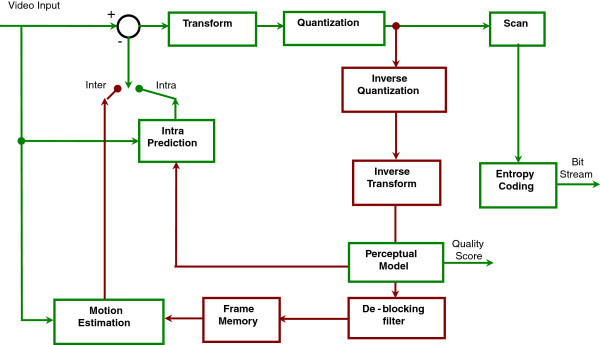
\includegraphics[scale=4.0]{img/h264.jpg} 
    \end{center}
\end{minipage}



\section{gstreamer}

Wenn Fehler beim Compilieren eines gstream Testprogramms auftreten, z.B.
\begin{verbatim}
Package gstreamer-1.0 was not found in the pkg-config search path.
Perhaps you should add the directory containing `gstreamer-1.0.pc'
to the PKG_CONFIG_PATH environment variable
No package 'gstreamer-1.0' found
playback-tutorial-6.c:1:10: fatal error: gst/gst.h: No such file or directory
\end{verbatim}

gstreamer-1.0 ist der folgenden lib enthalten:\\
sudo apt install libgstreamer1.0-dev\\

\textbf{Beispiel Programme gstreamer kompilieren}
gcc playback-tutorial-6.c -o playback-tutorial-6 `pkg-config --cflags --libs gstreamer-1.0`

\section{Strato Web Server}

\textbf{Login via ssh}\\
ssh -X root@85.214.211.169\\
ssh -X root@85.214.211.169 -L 5901:localhost:5901\\
pwd: xxxxxxxxxx (pwd vom Provider)

\textbf{Remote Desktop}\\
tightvncserver: server\\
xtightvncviewer: viewer\\
sudo apt install tightvncserver xtightvncviewer\\
\# set xtightvnciewer pwd\\

\textbf{Full Login}\\
ssh -X root@85.214.211.169 -L 5901:localhost:5901\\
ssh Passwort eingeben\\
\# Start vncserver\\
vncserver :1\\
echo \grqq{}\$DISPLAY\grqq{}\\
\# in server ssh console\\
xtightvncviewer 127.0.0.1:1\\
vnc Passwort eingeben\\
\# X Fenster sollte sich öffnen







